\documentclass[../main.tex]{subfiles}

\begin{document}
\section{Aplicabilidad de la Identidad Autosoberana}\label{Aplicabilidad de la Identidad Autosoberana}
Analizando la situación actual descrita en el \hyperref[Estado del arte]{Estado del arte}, resulta notable que tanto el paradigma en sí mismo como su adaptación al gran público europeo mediante la \acrshort{eIDAS} traten de \textbf{reflejar} la información de entidades reales (entorno físico) a su equivalente digital. 
\\

De igual manera que se puede gestionar las credenciales, gracias al paradigma de la \acrshort{SSI} el conjunto de dispositivos del \acrfull{IoT} es capaz de autenticarse y almacenar información referente a ellos mediante sus propios \textbf{certificados} (\acrshort{VC} para objetos).

\refstepcounter{observacion}
\begin{tcolorbox}[colback=gray!10!white, colframe=gray!50!black, title=Observación \theobservacion]\label{observacion-IoT}
Cuando hablamos de dispositivos del \acrshort{IoT} nos referimos a todo aquel que sea capaz de conectarse a la red Wi-Fi, que tenga una manera de identificarse inequívocamente en ella y que posea la funcionalidad de recoger información del entorno para su procesamiento. Ejemplos: Sensores, cámaras de vigilancia, teléfonos inteligentes, electrodomésticos ...
\end{tcolorbox} 

Por este motivo, la \acrfull{ITN} propone el uso de un nuevo término para referirse al \acrshort{DT} de los dispositivos del \acrshort{IoT} para así destacar el aspecto descentralizado del proceso de identificación, al que denominan \acrfull{SSDT} \cite{IOTinSSI}. 
\noindent Estos tendrán la capacidad de expedir, gestionar y consultar (dependiendo del actor) sus certificados mediante un único \textbf{registro} que haga las veces de \acrshort{VDR}, mantenido por la propia \acrshort{ITN} \cite{IOTinSSI_DIDs} siguiendo la misma idea propuesta por la \acrshort{EBSI} para la implantación de la \acrshort{eIDAS}. 
\\

%\begin{figure}[htbp]
%    \centering
%    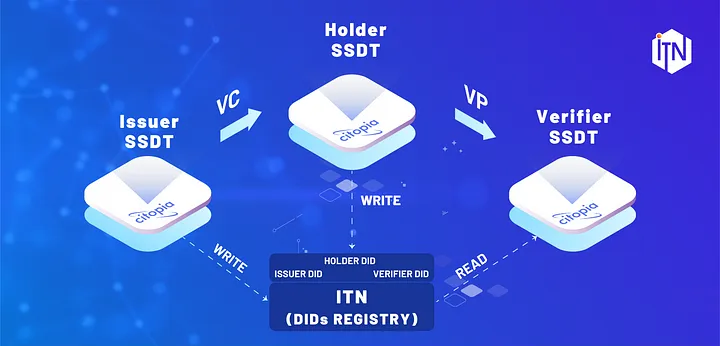
\includegraphics[width=0.7\linewidth]{images/SSDT_Actores.png}
%    \caption{\textit{Actores y sus funciones en los \acrshort{SSDT}s.} Fuente \cite{IOTinSSI_DIDs}}
%    \label{fig:actores}
%\end{figure}

%la aplicación a otros paradigmas novedosos requieren de un análisis más detallado.
Como se ha podido comprobar, el paradigma de la \acrshort{SSI} tiene la capacidad de ser aplicado en múltiples ámbitos igualmente innovadores con los que comparte fundamentos. De hecho, el alcance de esta situación es tal que 
\\

Por lo tanto, el presente estudio debe expandirse hasta abarcar el área de \hyperref[Gemelos Digitales]{Gemelos Digitales} para así conocer los \hyperref[Riesgos y amenazas]{Riesgos y amenazas} intrínsecos al emplear el paradigma como alternativa a la centralización. Además, con el objetivo de completar el análisis teórico previo desde un punto de vista práctico, se elaborará una \hyperref[Prueba de concepto]{Prueba de concepto} en la que se implementarán los componentes técnicos necesarios para reproducir el sistema en un entorno lo más real posible.
\\

% -----------------
% Gemelos Digitales
% -----------------
\subsection{Gemelos Digitales.}\label{Gemelos Digitales}
\subsubsection{Definición del concepto.}\label{Definición del concepto}
El concepto de \acrfull{DT} como lo conocemos actualmente tiene multitud de pequeñas variaciones según el contexto en el que se emplee y el aspecto a destacar del mismo, aunque no debe ser confundido con términos como \Gls{Simulador}, \Gls{Avatar Digital} o \Gls{Huella Digital}. 
\\

Algunos ejemplos de entornos digitalizables son el \textbf{industrial} mediante la replicación del proceso de producción, el \textbf{sanitario} con el modelado del estado de los pacientes o el \textbf{civil} para la creación de ciudades inteligentes tras monitorizar aspectos como el tráfico. Un caso en el que se puede ver hasta donde se puede extrapolar esta idea es en los esfuerzos por parte de NVIDIA en crear un \acrshort{DT} de la Tierra para simular el efecto del cambio climático \cite{Earth_NVIDIA}.
\\

\newpage
De tal manera, en el contexto de este escrito definiremos el concepto como ``una representación virtual de un componente o sistema físico'' \cite{DT_NVIDIA}, en el que se sobrentiende que tratamos de digitalizar la identidad de la persona mediante la creación de las \acrshort{VC}s. En otras palabras, podemos decir que llegados a este punto del paradigma hemos derivado a un entorno de \acrshort{DT}s ya que son igualmente distinguibles la propia persona \textbf{física} como su contraparte \textbf{digital}. 
\\

También es posible entenderlo de manera inversa, puesto que su capacidad de ``caracterizar activos físicos a través de activos digitales'' \cite{ThreatsDT} hace resaltar la fuerte conexión que ambas partes han de mantener. Cualquier creación, actualización o eliminación de información en una de las  partes debe verse reflejada en su equivalente para mantener siempre la concordancia.
\\

% -------------------
% Espacios de trabajo
% -------------------
\subsubsection{Espacios de trabajo.}\label{Espacios de trabajo}

Siguiendo esta distinción, en el contexto de la \acrshort{SSI} podemos encontrar:

\begin{itemize}
    \item \textbf{Espacio Físico}, ámbito de los activos físicos. \\
    A él pertenecen aquellos mecanismos como los \acrshort{VDR}s, las Carteras de Identidad Digital o los \acrshort{DID}s y sus derivados, cuya función consiste en modelar digitalmente los métodos tradicionales para la expedición de credenciales como DNIs, pasaportes, títulos educativos o cualquier otro tipo de documento acreditativo.

    \item \textbf{Espacio Digital}, ámbito de los activos digitales. \\
    Una vez nos desprendemos de la naturaleza real (soporte físisco) de la credencial mediante el uso de dichas herramientas, vemos que las \acrshort{VC}s son capaces de realizar la misma función sin sustituir a su contraparte, puesto que ambos trabajan en espacios diferentes. 
    
\end{itemize}

Determinados autores como \cite{ThreatsDT} añaden a esta separación entre espacios un tercero al que denominan como ``\textbf{Espacio de Comunicación}'' que interconecta a ambos. Conformado por interfaces o servicios que manejasen los datos, en nuestro contexto se correspondería con el escenario conformado por los \hyperref[Actores y sus funciones en el paradigma]{actores} del paradigma, con sus relaciones y el uso que dan a sus dispositivos en los que guardan sus Carteras de Identidad Digital.


% ----------------------
% Arquitectura multicapa
% ----------------------
\newpage
\subsubsection{Arquitectura multicapa.}\label{Arquitectura multicapa}
En \cite{ThreatsDT} se realiza una completa labor de investigación que resulta en la definición de una arquitectura de un total de cuatro \textbf{capas de funcionalidad} para los sistemas de \acrshort{DT}s:
\\

\begin{itemize}
    \item \textbf{Capa 1}, \textit{difusión y adquisición de datos}. 
    \\ Es la capa más cercana al espacio físico y por ello interactúa directamente con los activos físicos. No solo tiene a cargo la recopilación de datos mediante \textbf{sensores} que envía a las capas superiores, sino que también posee \textbf{actuadores} con los que transmite la respuesta recibida para mantener la consistencia entre ambos activos.
    \\
    
    \item \textbf{Capa 2}, \textit{gestión y sincronización de datos}.
     \\ Previo al uso de estos datos heterogéneos (probablemente obtenidos de diversas fuentes) recibidos de la capa anterior, se debe realizar una serie de procesos de \textbf{normalización} y \textbf{enriquecimiento} que mejoren el rendimiento de los servicios de la tercera capa. Igualmente, se ha de controlar de forma \textbf{sincronizada} el flujo de información en ambos sentidos para lograr una correcta comunicación en la red. 
     \\
    
    \item \textbf{Capa 3}, \textit{modelado de datos y servicios adicionales}. 
    \\ La capa principal del la arquitectura es la encargada de, a través de modelos digitales creados a partir de los activos físicos y gracias a la información proporcionada, especificar los \textbf{estados} y \textbf{comportamientos} de estos para así poder analizar escenarios sin interferir en el mundo físico. Esto es posible mediante \textbf{servicios} que junto con la acción de los \textbf{sensores y actuadores virtuales} permiten la definición de los activos digitales.
    \\ 

    \item \textbf{Capa 4}, \textit{visualización de datos y accesibilidad}. 
    \\ Como su nombre bien indica, facilita a los usuarios la consulta de los resultados obtenidos tras el modelado para la toma de decisiones. Otros mecanismos pueden ser definidos, como la gestión de la cadena de suministro o tener múltiples \acrshort{DT}s en el mismo sistema.
    \\
\end{itemize}

\begin{figure}[htbp]
    \centering
    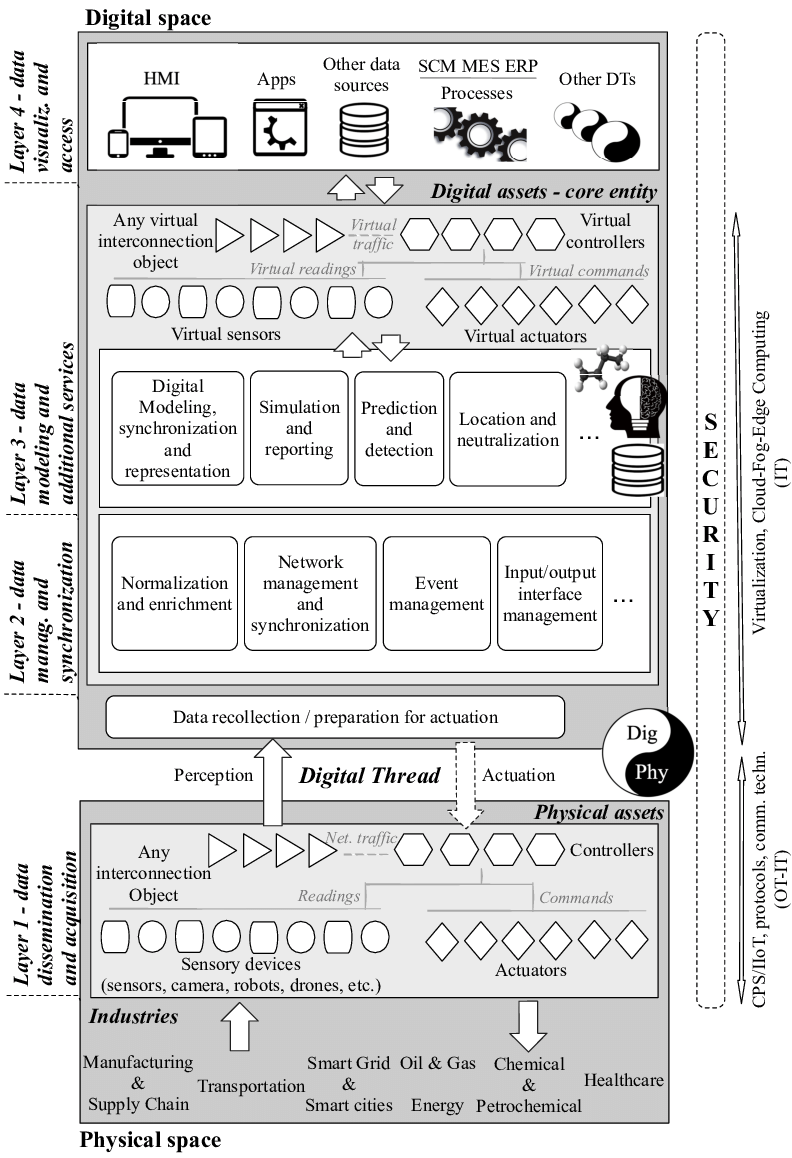
\includegraphics[width=0.8\linewidth]{images/DT_Layers.png}
    \caption{\textit{Arquitectura multicapa para los \acrshort{DT}s.} Fuente \cite{ThreatsDT}}
    \label{fig:capas}
\end{figure}


% ------------------
% Riesgos y amenazas
% ------------------
\newpage
\subsection{Riesgos y amenazas.}\label{Riesgos y amenazas} 
Una vez definida, es posible hacer uso de la \hyperref[Arquitectura multicapa]{arquitectura multicapa} como base para \textbf{asociar} las vulnerabilidades propias de la \acrshort{SSI} con las intrínsecas de \acrshort{DT}s. Así pues, se realizará un análisis conjunto de su aplicabilidad para componentes y activos digitales. Las principales fuentes de información empleadas para la elaboración de esta sección son \cite{ThreatsDT} para el ámbito de los \acrshort{DT}s, además de \cite{ChallengesSSI} y \cite{ThreatModeling} para el paradigma de la \acrshort{SSI}. 


% ------
% Capa 1
% ------
\subsubsection{Capa 1, difusión y adquisición de datos.}
\begin{enumerate}[label=\textbf{R1.\arabic*}, leftmargin=48pt]
    % ------ R1.1
    \item \textbf{Vulnerabilidades propias de la Blockchain.}\label{R1.1}
    \\ Los \acrshort{VDR}s garantizan la descentralización y transparencia al paradigma, pero son susceptibles a ataques a mecanismos propios como los \Gls{contratos inteligentes}, ya sea explotando vulnerabilidades, desactivándolos, o cambiando las configuraciones.

    \underline{Amenazas relacionadas en el ámbito de los \acrshort{DT}s}:
    \begin{itemize}
        \item \textbf{Escalado de privilegios [A1.1]:}\label{A1.1}
        \\ Los atacantes sortearían la seguridad que la Blockchain proporciona si logran tomar el papel de administradores del \acrshort{VDR} (o suplantar a otros actores) y así tener la capacidad de realizar acciones maliciosas de forma encubierta.
        \item \textbf{Denegación de servicio (DoS) [A1.2]:}\label{A1.2}
        \\ El sistema es susceptible a ser saturado por peticiones benignas o maliciosas que en su conjunto supongan un problema para ser atendidas. Esto afectaría a la gestión del espacio físico y por tanto, a la creación de los activos digitales.
    \end{itemize}
    
    \underline{Amenazas mitigadas en el ámbito de los \acrshort{DT}s}: 
    \begin{itemize}        
        \item \textbf{Daño físico [A1.3]:}\label{A1.3} 
        \\ La principal cualidad de la Blockchain es la descentralización, puesto que su división en nodos permite la distribución de la información. Los protocolos de consenso garantizan que, si alguno de sus nodos ha sido vulnerado, los cambios propuestos por él no sean efectuados ya que el resto discreparía. No obstante, si el número de máquinas vulneradas es mayor al establecido (Quórum) se perdería esta barrera de seguridad y existiría riesgo de manipulación en el sistema.
    \end{itemize}

    % ------ R1.2
    \item \textbf{Suplantación de la identidad digital.}\label{R1.2}
    \\ Aunque los mecanismos técnicos permiten afirmar de forma descentralizada que el portador de las \acrshort{VC}s es quién dice ser, esto no garantiza que existan métodos para aprovechar esa asociación con fines maliciosos. De entre ellos, podemos destacar la obtención/eliminación de la clave privada o el aprovechamiento de los métodos de recuperación de la identidad. 

    \underline{Amenazas relacionadas en el ámbito de los \acrshort{DT}s}:
    \begin{itemize}
        \item \textbf{Extracción de información privada [A1.4]:}\label{A1.4}
        \\ Si el dispositivo en el que se almacena la información sensible necesaria para la correcta identificación del usuario (como su clave privada o las propias \acrshort{VC}s) resulta vulnerado, no existe ningún aspecto técnico que impida al atacante a usurpar su identidad. Esto puede evitarse mediante una correcta protección del dispositivo, como una buena política de contraseñas, usar la identificación biométrica o tener activado la \Gls{2FA}.
    \end{itemize}
    
    \underline{Amenazas mitigadas en el ámbito de los \acrshort{DT}s}: 
    \begin{itemize}
        \item \textbf{Man-in-the-middle [A1.5]:}\label{A1.5}
        \\ La identificación de los actores pertenecientes al espacio de comunicación es fundamental en este paradigma. Todos los mecanismos técnicos tienen como razón de ser alegar la identidad digital de los miembros mediante sus \acrshort{DID}s consultables, garantizando que el contacto sea directo entre las partes. 
        \\
    \end{itemize}

    % ------ R1.3
    \item \textbf{Vulneración de la soberanía del dispositivo.}\label{R1.3}
    \\ En la misma línea que la vulnerabilidad anterior, es de recalcar la vital importancia que el dispositivo tiene en el paradigma como almacén de las \acrshort{VC}s. Aquel con acceso al mismo tiene el control de la identidad digital del usuario y a todos los efectos actúa como `él' de manera reconocida y oficial en los entornos digitales que apliquen. 
    
    Por este motivo, cualquier acción maliciosa sobre su dispositivo es un ataque directo a su identidad digital, como por ejemplo el robo, la manipulación de los métodos de acceso o la inutilización física deliberada.   

    \underline{Amenazas relacionadas en el ámbito de los \acrshort{DT}s}:
    \begin{itemize}
        \item \textbf{Ataque al software [A1.6]:}\label{A1.6}
        \\ El uso de software de terceros puede introducir vulnerabilidades al paradigma. Estas dependencias, incluidas como librerías o desarrolladas en el código para implementar algún componente (como la \acrshort{EUDI Wallet}), también son propicias a ocasionar errores o generar alteraciones en el funcionamiento del sistema. 
        \item \textbf{Dispositivos maliciosos [A1.7]:}\label{A1.7}
        \\ Una vez comprometido, el dispositivo se convierte en la mejor manera para modificar el estado del \acrshort{DT}, es decir, el atacante puede hacer y deshacer sin ningún impedimento en todo aspecto relativo a la identidad digital del usuario. Esto incluye la creación y eliminación de \acrshort{VC}s, establecimiento de autorizados o el uso fraudulento de la misma en sitios o formas indeseadas. 
        \item \textbf{Manipulación de hilos digitales [A1.8]:}\label{A1.8}
        \\ Un caso concreto de la amenaza anterior es la introducción de código malicioso, configuraciones erróneas o datos falsos para producir una desincronización del espacio físico y afectar así al espacio digital, puesto que ambos mantienen una robusta relación. El eslabón débil es nuevamente la Cartera de Identidad Digital del usuario, la cual puede llegar a ser manipulada para hacer creer al usuario que el estado de su \acrshort{DT} es diferente al real.
    \end{itemize}
    
    \underline{Amenazas mitigadas en el ámbito de los \acrshort{DT}s}: 
    \begin{itemize}
        \item No aplican.
        \\
    \end{itemize} 
\end{enumerate}

\refstepcounter{analisis}
\begin{tcolorbox}[colback=gray!10!white, colframe=gray!50!black, title=Análisis de la Capa \theanalisis]\label{analisis-C1}
La Blockchain supone un gran avance para descentralizar la información necesaria para la identificación, pero no es capaz de solventar los problemas que ocasionaría el uso malintencionado (pero igualmente válido) de los mecanismos técnicos de la \acrshort{SSI}. 

Además, el dispositivo se convierte en pilar para la seguridad del sistema, haciendo más sencillo atacar el espacio físico que el digital (su protección queda en manos del usuario). 
\end{tcolorbox}


% ------
% Capa 2
% ------
\newpage
\subsubsection{Capa 2, gestión y sincronización de datos.}
\begin{enumerate}[label=\textbf{R2.\arabic*}, leftmargin=48pt]
    % ------ R2.1
    \item \textbf{Manipulación sobre los nodos de la red.}\label{R2.1}
    \\ Uno de los mayores retos para el paradigma de la \acrshort{SSI} es la escalabilidad en su uso. La implantación masiva para el gran público supondrá un grave problema para la sincronización de los datos, por lo que soluciones basadas en la nube o software de virtualización para el aislamiento del sistema tomarán mayor relevancia. 
    
    Este hecho incluirá inevitablemente nuevas vulnerabilidades al paradigma, las cuales se añadirán a las ya presentes durante el proceso de establecimiento de los mismos. Ejemplo de ello es la propagación de mensajes falsificados para forzar el cierre, reinicio o aislamiento de los nodos, sin la necesidad de penetrar en el sistema.

    \underline{Amenazas relacionadas en el ámbito de los \acrshort{DT}s}:
    \begin{itemize}
        \item \textbf{Ataque al software [A2.1]:}\label{A2.1}
        \\ El despliegue de los nodos de la red en la nube o mediante software de virtualización puede ocasionar los mismos tipos de problemas mencionados en \hyperref[A1.6]{A1.6}. Además de las dependencias de la tecnología empleada, se introducen otras propias del sistema operativo sobre el que se realiza el despliegue (Windows o Linux). En el caso de las aplicaciones móviles también habría que considerar Android e IOS, como es el caso de la \acrshort{EUDI Wallet}.
        \item \textbf{Daño físico [A2.2]:}\label{A2.2}
        \\ Los atacantes pueden comprometer el estado de las \acrshort{VC}s tras tomar el control del sistema anfitrión, ya que podrían acceder a recursos sensibles, modificar configuraciones, parar servicios o ejecutar código. Sin embargo, los ataques a los servidores que conforman la nube resultan inusuales debido a la robusta capacidad de defensa que estos suelen poseen.
        \item \textbf{Escalado de privilegios [A2.3]:}\label{A2.3}
        \\ Puede ser tentador para los atacantes realizar acciones maliciosas en el sistema que requieran privilegios elevados, como tomar el control del sistema anfitrión. Este hecho también aplica al software de virtualización, haciendo que el acceso directo sea una verdadera amenaza.
        \item \textbf{Nodos maliciosos [A2.4]:}\label{A2.4}
        \\ De igual manera, si un nodo se ha visto comprometido puede actuar con fines maliciosos en la red realizando modificaciones del estado interno del mismo o denegando su operabilidad  (reduciendo el número de nodos activos). Por los motivos descritos en \hyperref[A1.3]{A1.3}, esto no supondría un riesgo para un número pequeño de nodos pero que podría ocasionar alteraciones graves en la red si aumenta.
    \end{itemize}
    
    \underline{Amenazas mitigadas en el ámbito de los \acrshort{DT}s}: 
    \begin{itemize}
        \item \textbf{Pérdida de privacidad [A2.5]:}\label{A2.5}
        \\ Esta amenaza hace referencia al uso indebido que las grandes corporaciones pueden llegar a hacer con los datos personales de sus usuarios, normalmente incorporando a su modelo de negocio la venta a terceros o el uso de técnicas computacionales para realizar análisis de mercado. 
        
        El paradigma de la \acrshort{SSI}, como alternativa descentralizada que es, no requiere del uso de estos servicios más allá de los motivos descritos en esta sección. Además, gracias a la transparencia que supone reflejar información `sensible' en la Blockchain pública, la cantidad de datos privados se ve reducida.
        \\
    \end{itemize}
    
    % ------ R2.2
    \item \textbf{Ataque al espacio de comunicación.}\label{R2.2}
    \\ Debido a que los grandes proveedores de servicios en la nube suelen ser demasiado seguros y como la solución que propone el paradigma de la  \acrshort{SSI} resulta ser lo suficientemente robusta, los principales vectores de ataque se concentran en los puntos de transmisión y recepción de datos. En este caso, el objetivo son los propios actores.
    
    \underline{Amenazas relacionadas en el ámbito de los \acrshort{DT}s}:
    \begin{itemize}
        \item \textbf{Man-in-the-middle [A2.6]:}\label{A2.6}
        \\ En toda comunicación llevada a cabo sobre una infraestructura de red existe la posibilidad de interceptación de los mensajes compartidos entre los actores. Esto puede ser evitado mediante el establecimiento de conexiones seguras, el empleo de mecanismos de cifrado para ocultar el contenido de los mensajes y el uso responsable del medio, evitando compartir información sensible.
        \item \textbf{Extracción de información privada [A2.7]:}\label{A2.7}
        \\ Siguiendo la misma línea descrita en \hyperref[A2.3]{A2.3}, si el usuario decide alojar en la nube su Cartera de Identidad Digital (la cual contiene sus \acrshort{VC}s) o aislarla mediante un software de virtualización, existe la posibilidad que los administradores o usuarios privilegiados del sistema anfitrión realicen una labor de monitorización sobre sus comunicaciones e interceptar información sensible.
        \item \textbf{Denegación de servicio (DoS) [A2.8]:}\label{A2.8}
        \\ Ante el impedimento de utilizar los servicios para acceder a los recursos necesarios para la identificación, independientemente de si han sido almacenados de manera local, en la nube o en una máquina virtual, el usuario no podría utilizarlos aún siendo el poseedor de las \acrshort{VC}s allí alojadas. Por lo tanto, a efectos prácticos perder el acceso supone `dejar de ser' digitalmente hablando. 
    \end{itemize}
    
    \underline{Amenazas mitigadas en el ámbito de los \acrshort{DT}s}: 
    \begin{itemize}
        \item No aplican.
        \\
    \end{itemize} 
\end{enumerate}

\refstepcounter{analisis}
\begin{tcolorbox}[colback=gray!10!white, colframe=gray!50!black, title=Análisis de la Capa \theanalisis]\label{analisis-C2}
El papel que realizan los componentes de esta capa seguramente sea el más complicado de lograr de manera segura, puesto que ninguno de los dos paradigmas solventan de manera efectiva la sincronización de los nodos de la red. 
\\

De hecho, uno de los puntos fuertes de la \acrshort{SSI} es su robustez ante las acciones maliciosas que intentan `romper' sus métodos criptográficos, pero esta resultaría sorteada si se obtiene acceso a toda la \acrshort{VC} (o incluso al \acrshort{DID}) para así usurpar la identidad.  
\\

Sucede algo parecido con la \Gls{2FA}, puesto que es más seguro si los códigos están asociados a un único dispositivo local sobre el que se tiene control absoluto. No obstante, sería correcto destacar que estos tienen un propósito diferente y carecen del fuerte aspecto interactivo que poseen las \acrshort{VC}s.
\end{tcolorbox}


% ------
% Capa 3
% ------
\newpage
\subsubsection{Capa 3, modelado de datos y servicios adicionales.}
\begin{enumerate}[label=\textbf{R3.\arabic*}, leftmargin=48pt]
    % ------ R3.1
    \item \textbf{Uso fraudulento de las \acrshort{VC}s.}\label{R3.1}
    \\ A pesar de la fortaleza que los mecanismos técnicos de la \acrshort{SSI} muestran, resultan  ser insuficientes para evitar la manipulación o el uso malicioso por parte de atacantes.

    \underline{Amenazas relacionadas en el ámbito de los \acrshort{DT}s}:
    \begin{itemize}
        \item \textbf{Ataque al software [A3.1]:}\label{A3.1}
        \\ Durante el proceso de creación, modificación y eliminación de las \acrshort{VC}s es posible que se cometan errores que introduzcan vulnerabilidades al sistema desde el espacio digital. Esta idea sigue la misma línea descrita en \hyperref[A1.6]{A1.6}.
        \item \textbf{Extracción de información privada [A3.2]:}\label{A3.2}
        \\ Tal y como se menciona en \hyperref[A2.7]{A2.7}, si el atacante llega a tomar control de las \acrshort{VC}s toda su potencial información privada que contengan puede ser extraída, incluyendo datos personales y referencias a credenciales físicas.
        \item \textbf{Pérdida de privacidad [A3.3]:}\label{A3.3}
        \\ Vulnerando múltiples \acrshort{VC}s de un mismo usuario, es posible correlacionar la información que contienen para inferir relaciones o asociaciones que puedan llegar a comprometer su privacidad.
    \end{itemize}
    
    \underline{Amenazas mitigadas en el ámbito de los \acrshort{DT}s}: 
    \begin{itemize}
        \item \textbf{Manipulación de los datos contenidos [A3.4]:}\label{A3.4}
        \\ Puesto que las \acrshort{VC}s poseen mecanismos que preservan la integridad de los datos, la posibilidad de alterar su contenido para su posterior uso se ve invalidada. 
        \\
    \end{itemize}
\end{enumerate}

\refstepcounter{analisis}
\begin{tcolorbox}[colback=gray!10!white, colframe=gray!50!black, title=Análisis de la Capa \theanalisis]\label{analisis-C3}
Es destacable que la mejor manera para afectar al espacio digital sea mediante las capas anteriormente descritas. Una vez ha sido creada, la \acrshort{VC} supone un punto de inflexión en la arquitectura del paradigma y pasan a ser un objetivo para los atacantes, los cuales tratarán de obtener toda información posible que esté contenida en ellas. 


\end{tcolorbox}

% ------
% Capa 4
% ------
\newpage
\subsubsection{Capa 4, visualización de datos y accesibilidad.}
\begin{enumerate}[label=\textbf{R4.\arabic*}, leftmargin=48pt]
    % ------ R4.1
    \item \textbf{Distorsión de los datos en su representación.}\label{R4.1}
    \\ En última instancia encontramos que, ante las protecciones que el sistema puede poseer para evitar la manipulación de los activos físicos (e incluso digitales), resulte tentador para los atacantes dirigir sus esfuerzos a comprometer la impresión del estado de las \acrshort{VC}s para así aprovechar otras vulnerabilidades.

    \underline{Amenazas relacionadas en el ámbito de los \acrshort{DT}s}:
    \begin{itemize}
        \item \textbf{Ataque al software [A4.1]:}\label{A4.1}
        \\ Atacando directamente los componentes de la aplicación que muestra las \acrshort{VC}s al usuario, se puede alterar el comportamiento de la misma sin la necesidad de haber afectado al funcionamiento de los mecanismos técnicos de la \acrshort{SSI}.
        \item \textbf{Manipulación de la visualización de los datos [A4.2]:}\label{A4.2}
        \\ Un caso particular de la amenaza anterior es, tras afectar a la correcta visualización de la información, originar en los usuarios ideas equivocadas que inciten a realizar acciones innecesarias. Para lograrlo, los atacantes pueden mostrar los datos de manera errónea e inconsistente, esconder determinada información o afectar la integridad de la misma.
    \end{itemize}
    
    \underline{Amenazas mitigadas en el ámbito de los \acrshort{DT}s}: 
    \begin{itemize}
        \item \textbf{Aplicaciones maliciosas [A4.3]:}\label{A4.3}
        \\ Gracias a soluciones de código abierto como la \acrshort{EUDI Wallet}, el notable riesgo que supondría tener múltiples métodos de gestión de las \acrshort{VC}s se ve reducido. Esto es no solo por establecer una única aplicación para su uso generalizado, sino por mantener la descentralización al almacenarlas en los dispositivos. 
        \\
    \end{itemize}
\end{enumerate}

\refstepcounter{analisis}
\begin{tcolorbox}[colback=gray!10!white, colframe=gray!50!black, title=Análisis de la Capa \theanalisis]\label{analisis-C4}
El principal riesgo asociado a esta capa es el engaño por parte de la aplicación al usuario. 

Además, comprobamos cómo la confianza puesta sobre la correcta implementación de la aplicación es máxima, por lo que toda transparencia posible resulta agradecida.  
\end{tcolorbox}


% -------------------------------
% Balance general y tabla resumen
% -------------------------------
\newpage
\subsubsection{Balance general y tabla resumen.}\label{Balance general y tabla resumen}
Tras este intento por adecuar el paradigma de la \acrshort{SSI} en un entorno de \acrshort{DT}s, en el que se ha fusionado las capas de ambos ámbitos para analizar sus riesgos y amenazas, recopilamos las conclusiones obtenidas a lo largo del mismo para destacar que: 

\begin{itemize}
    \item Las principales vulnerabilidades surgen entre la \textbf{capa 1 y 2}. 
    \item Están relacionadas con la \textbf{implementación} a nivel de software y comunicaciones. 
    \item Los mecanismos técnicos de la \acrshort{SSI} mitigan \textbf{algunas} de estas amenazas.
    \item Existen grandes \textbf{similitudes} entre ambos paradigmas en estos aspectos.
\end{itemize}
A continuación se detalla la tabla resumen que recoge el análisis realizado: 
\\

\setlength{\tabcolsep}{0.5em} 
\renewcommand{\arraystretch}{1.5}
\begin{table}[h!]
    \begin{tabular}{|p{1.5cm}||p{3cm}|p{2.5cm}|p{3.8cm}|p{3cm}|}
        \hline
        & 
        \textbf{Aspecto \newline vulnerado} & 
        \textbf{Riesgo \acrshort{SSI} \newline intrínseco} & 
        \textbf{Amenazas \acrshort{DT} \newline relacionadas} &
        \textbf{Amenazas \acrshort{DT} \newline mitigadas} \\
        \hline\hline
        
        \textbf{Capa 1} & 
        \acrshort{VDR} & 
        \hyperref[R1.1]{R1.1} &
        \hyperref[A1.1]{A1.1}, \hyperref[A1.2]{A1.2} &
        \hyperref[A1.3]{A1.3}  \\
        \cline{2-5} & 
        Cartera de \newline Identidad Digital  & 
        \hyperref[R1.2]{R1.2} \newline \hyperref[R1.3]{R1.3} & 
        \hyperref[A1.4]{A1.4} \newline \hyperref[A1.6]{A1.6}, \hyperref[A1.7]{A1.7}, \hyperref[A1.8]{A1.8} &
        \hyperref[A1.5]{A1.5} \newline No aplican \\
        \hline
        
        \textbf{Capa 2} & 
        Nodo de la red & 
        \hyperref[R2.1]{R2.1}  & 
        \hyperref[A2.1]{A2.1}, \hyperref[A2.2]{A2.2}, \hyperref[A2.3]{A2.3}, \hyperref[A2.4]{A2.4} &
        \hyperref[A2.5]{A2.5} \\
        \cline{2-5} & 
        Comunicaciones & 
        \hyperref[R2.2]{R2.2}  & 
        \hyperref[A2.6]{A2.6}, \hyperref[A2.7]{A2.7}, \hyperref[A2.8]{A2.8} &
        No aplican \\
        \hline
        
        \textbf{Capa 3} & 
        \acrshort{VC} & 
        \hyperref[R3.1]{R3.1} &  
        \hyperref[A3.1]{A3.1}, \hyperref[A3.2]{A3.2}, \hyperref[A3.3]{A3.3} &
        \hyperref[A3.4]{A3.4} \\
        \hline
        
        \textbf{Capa 4} & 
        Representación & 
        \hyperref[R4.1]{R4.1} & 
        \hyperref[A4.1]{A4.1}, \hyperref[A4.2]{A4.2} &
        \hyperref[A4.3]{A4.3} \\
        \hline
    
    \end{tabular}
 \caption{Asociación de los riesgos y amenazas en el conjunto de ambos paradigmas.}
 \label{tabla_amenazas}
\end{table}


% ------------------
% Prueba de concepto
% ------------------
\newpage
\subsection{Prueba de concepto.}\label{Prueba de concepto}
\subfile{sections/PruebaDeConcepto}

\end{document}